\chapter{Impact of Changes on MEP Systems}
\section{Introduction  \label{HVAC}}
\begin{marginfigure}%
  \includegraphics[width=\linewidth]{plantrooms}
  \caption{On the 31$^{st}$ March 2010, HOK issues EI-454AM, which instructs HEE to relocate the chilled water
pump and add double doors for better access and maintenance in plant
room ROB313A, TRO LB3. The change affected completion of Qatar Cool Plantrooms.}
  \label{fig:marginfig1}
\end{marginfigure}
\begin{marginfigure}%
  \includegraphics[width=\linewidth]{watertanks}
  \caption{Primary co-ordination issues affected all aspects of MEP works. The photo, shows the \textit{digging of slabs} to provide access on top of water tanks in Level 5. Many of these tanks were located underneath, AHU plinths.}
  \label{fig:marginfig1}
\end{marginfigure}
\begin{marginfigure}%
 \includegraphics[width=\linewidth]{./graphics/AHU/watertanks}
  \caption{On Level 4, water tanks, just fit in the volume provided. No space for access on top is possible. }
  \label{fig:marginfig1}
\end{marginfigure}

\newthought{With more than 94 units affected by Engineering Instructions} works were impacted in all areas. A graphical overview of the equipment impacted is shown in figures 1-10, where all clouded areas show equipment that were affected. No area in the Podia was not affected by these changes, from the smaller store to the largest areas such as ballrooms. For the Towers changes mostly affected higher floors and Restaurants. Other changes that followed from these were demolition of plantroom walls to re-arrangements in ceiling to accommodate the changes.

\subsection{Mitigation Measures} 

\subsubsection{Engineering Office}
When the Contractor realized that the Engineer did not had a complete design and the seriousness of the changes, he proceeded to boost his Engineering Office capacity in order to accelerate the works and achieve the interim milestones. HS arranged for its Design Manager Mr. Terry Green as well as a number of other Senior Design staff to spent approximately six months in Doha to complete the work necessary to implement the requested changes. It also boosted its drawing office capacity to 28 CAD Operators. 


\subsubsection{Labour Resource}

Similarly additional labour resources were employed both through local subcontractors and hired manpower to reach the levels, where works could be accelerated. 

\subsubsection{Wild Air}

As per the MOU the Contractor had to provide access to the Clients Fit-out Contractor at the end of June. Throughout this period the Engineer took the view that this meant to provide airconditioning in the form of `wild air'. A term that was not defined neither in the MOU nor in the Main Contract. For permanent installations this could be provided via a connection to Qatar Cool installations.
At this point a digression is necessary to review the necessary pre-conditions for such a connection.

\begin{enumerate}
\item The chilled water network had to be completed in its entirety.
\item Permanent power must be available.
\item A number of other requirements neither of which was unachievable within the original MOU dates.
\end{enumerate}


It will not be surprizing even to a person not conversant with MEP Services that the disruption and the ensuing productivity issues arising from such major changes affecting all areas, the completion of the Chilled Water netwrok in the podia was impossible to be achieved within the constraints of the agreed program. For the record changes to pipework continued with for example EI, with which we are still trying to finalize requirements with the Engineer.

For permanent Power to be achieved major cabling had to be installed throughout the ceiling voids of the Ground Floor and the main kitchen areas of Basement 1. Due to the highly congested nature of these ceiling voids, this was only possible once other services, such as installation of ceiling mounted air handling units, pipework and the like could be installed. In addition Electrical Boards in many areas had to be modified to accomodate the changes, electrical load schedules to be recalculated for submittal to the Engineer\sidenote{Drawings submitted in May 2010 to the Engineer have still to be reviewed and returned to the Contractor} and Kahraama for approval. 

The above is a brief overview, which to be appreciated must be read in conjuction to all the other chnages that have affected the works, including moving of walls in Merweb substation, adding doors to the Rotana Qatar Cool Plantroom (after equipment were installed), having to cut opening through slabs to access water tanks for which no adequate spaces were allowed). Many of these Engineer's Instructions were only issued to the Contractor beyond the \deadline, for example EI 479M dated 16th May 2010, RFI M-807, EI 554, RFI M-905 etc.

The Contractor realized that the changes experienced during the pre-MOU period were likely continued until the end of the Project took the decision to provide temporary installations for the provision of wild air. A plan was put into place and closely monitored. Wild air was provided to the Tower areas on the 28th of June for Rotana, 29th of June for Shangrila and 30th of June for Merweb.

The Client's Fit Out Contractor did not mobilize in July as expected. An appointment only having been made in late October 2010. An MEP Contractor for works in Restaurants - which are excluded in HEE's Contract is still to be made. As this is the first trade that has to be moved in when the Fitout Contractor is mobilized, it is apparent that the Project is on the path of further delays.



\section{Summary of Air handling Units affected by Changes}

The breadth of the changes and the impact to the HVAC and other trades was dramatic. Figure \ref{fig:RotanaAHUs} illustrates the percentage changes in Rotana. Some of the floors -- where ceiling void allowances -- were greatly underestimated in the Design, experienced changes upwards of 80\%. The Ground Floor 57\%. Floors such as Level 5, experienced 33\% change only because walls were demolished and the plantrooms increased in size.

\begin{figure}[htbp]
\centering
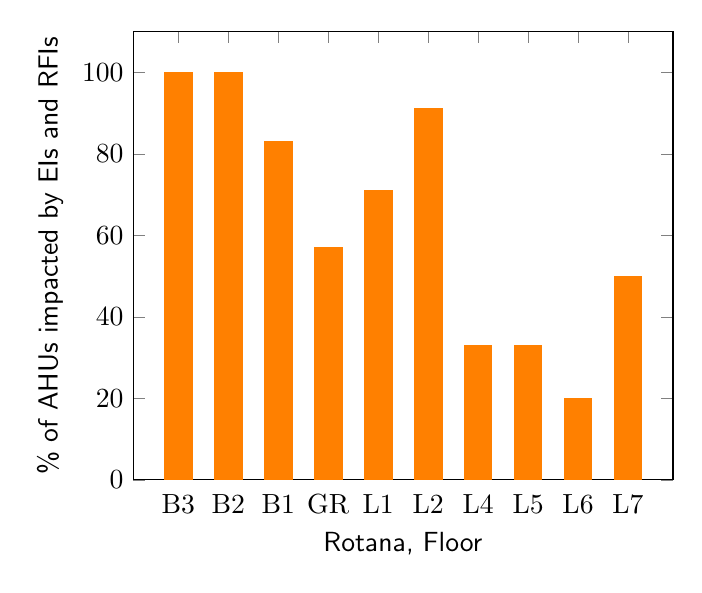
\begin{tikzpicture}
\begin{axis}[symbolic x coords={B3,B2,B1,GR,L1,L2,L4,L5,L6,L7},
xtick={B3,B2,B1,GR,L1,L2,L4,L5,L6,L7},  % Use this to decide which tickmarks to print
xticklabel style={text height=2ex}, % This aligns all letters on the same line, if it is missing, 'a' and 'b' are at different heights
ymin=0,
xlabel=\textsf{Rotana, Floor},
ylabel=\textsf{\% of AHUs impacted by EIs and RFIs},
] 

\addplot[color=orange,ybar,fill] coordinates {
(B3,100)
(B2,100)
(B1,83)
(GR,57)
(L1,71)
(L2,91)
(L4,33)
(L5,33)
(L6,20)
(L7,50)
 };

\end{axis}
\end{tikzpicture}
\caption{Rotana, percentage of AHUs affected by Engineer's 
Instructions or RFIs, by floor.}
\label{fig:RotanaAHUs}
\end{figure}

%% SHANGRILA
For Shangri-la a similar situation arose. The changes are graphically illustrated in Figure~\ref{fig:SLAHUs} and in more detail in Table . In a number of instances, such as the Fresh Air Handling Units located in Level 5, the Engineer kept on insisting to raise ducts and kept issuing FORs and NCRs for ducting to be raised. An impossible task (see Photo).

\begin{figure}[htbp]
\centering
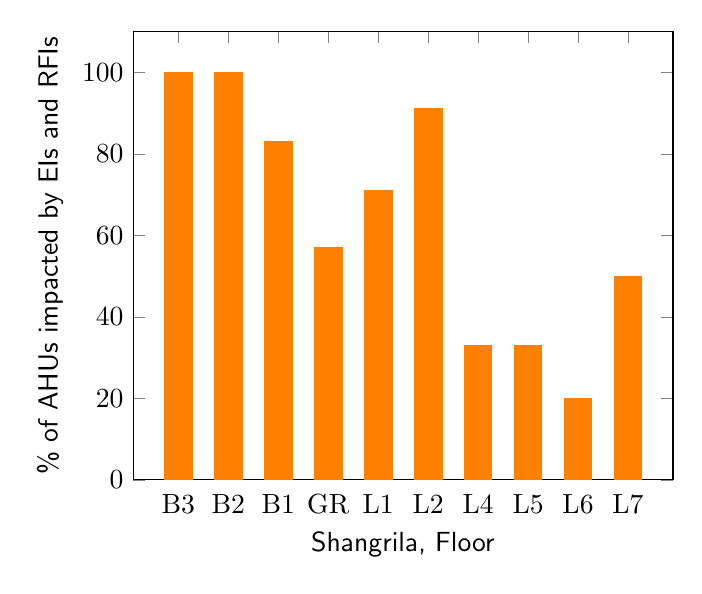
\begin{tikzpicture}
\begin{axis}[symbolic x coords={B3,B2,B1,GR,L1,L2,L4,L5,L6,L7},
xtick={B3,B2,B1,GR,L1,L2,L4,L5,L6,L7},  % Use this to decide which tickmarks to print
xticklabel style={text height=2ex}, % This aligns all letters on the same line, if it is missing, 'a' and 'b' are at different heights
ymin=0,
xlabel=\textsf{Shangrila, Floor},
ylabel=\textsf{\% of AHUs impacted by EIs and RFIs},
] 

\addplot[color=orange,ybar,fill] coordinates {
(B3,100)
(B2,100)
(B1,83)
(GR,57)
(L1,71)
(L2,91)
(L4,33)
(L5,33)
(L6,20)
(L7,50)
 };

\end{axis}
\end{tikzpicture}
\caption{Shangrila, percentage of AHUs affected by Engineer's 
Instructions or RFIs, by floor.}
\label{fig:SLAHUs}
\end{figure}


As Figure~\ref{fig:MWAHUs} clearly indicates, the Merweb Tower was affected in a similar manner. EIs were issued in a rushed manner, with no consideration whatsoever to maintenability, constructability costs or impacts to the overall construction program.

\begin{figure}[htbp]
\centering
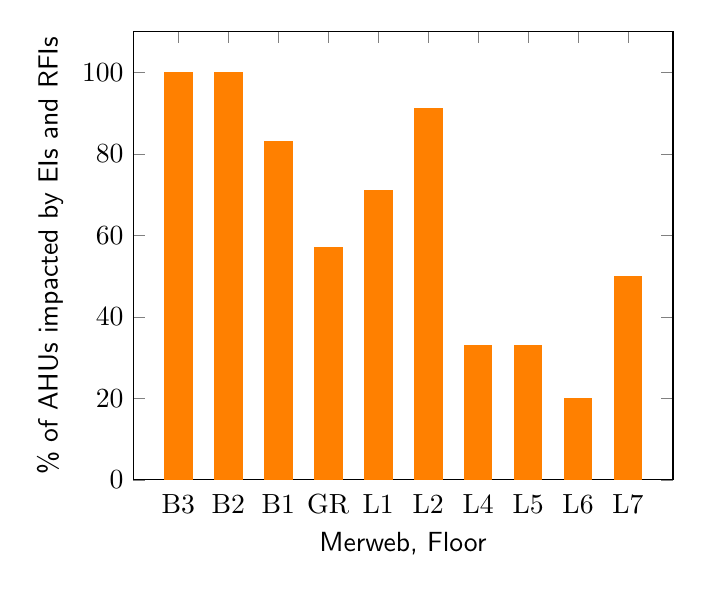
\begin{tikzpicture}
\begin{axis}[symbolic x coords={B3,B2,B1,GR,L1,L2,L4,L5,L6,L7},
xtick={B3,B2,B1,GR,L1,L2,L4,L5,L6,L7},  % Use this to decide which tickmarks to print
xticklabel style={text height=2ex}, % This aligns all letters on the same line, if it is missing, 'a' and 'b' are at different heights
ymin=0,
xlabel=\textsf{Merweb, Floor},
ylabel=\textsf{\% of AHUs impacted by EIs and RFIs},
] 

\addplot[color=orange,ybar,fill] coordinates {
(B3,100)
(B2,100)
(B1,83)
(GR,57)
(L1,71)
(L2,91)
(L4,33)
(L5,33)
(L6,20)
(L7,50)
 };

\end{axis}
\end{tikzpicture}
\caption{Merweb, percentage of AHUs affected by Engineer's 
Instructions or RFIs, by floor.}
\label{fig:MWAHUs}
\end{figure}



\newcounter{totalahu} \setcounter{totalahu}{0}
\newcounter{totaldeletedahu} \setcounter{totaldeletedahu}{0}

\newcounter{ro}
\setcounter{ro}{0}
\newcounter{rodel}
\setcounter{rodel}{0}
\def\inc{\stepcounter{ro}\thero\stepcounter{totalahu}}
\protect\def\deleted{\hl{deleted}\stepcounter{rodel}}
\protect\def\ROmodified{\hl{modified}\stepcounter{rodel}}
\protect\def\ROrelocated{\hl{relocated}\stepcounter{rodel}}

\def\ROAHU#1{\index{AHU Rotana!#1}#1}

\def\ROAHUD#1{\index{AHU Rotana!#1}\index{AHU Rotana, deleted!#1}#1}




\begin{table}[htbp]
\label{tbl:AHUrotana}
\footnotesize
\caption{Rotana Air Handling Unit installation changes. Deleted units (\therodel).}
\begin{tabular}{lll p{2cm}p{1.8cm}}
\toprule
Ref.	  &AHU tag 	 &Area	 &Installed	  &Date\\
\midrule
%%B2
\inc   &\ROAHUD{B2-RO-AH-1}   &District Cooling &  &\deleted\\	
\inc	  &\ROAHU{B2-RO-AH-2}	 &District Cooling Room &No	 &\deleted\\
\midrule 

%%B1
\inc	 &\ROAHU{B1-RO-AH-1} & n/a	         & deleted at design	 &\deleted\\
\inc	 &\ROAHU{B1-RO-AH-2} &Main Kitchen	         & Yes	 	 &\ROmodified\\
\inc	 &\ROAHU{B1-RO-AH-3}	 &BMS/ENG	 &Yes	 	                         &\ahufour\\
\inc    &\ROAHUD{B1-RO-AH4}   &Housekeeping                    &            &\deleted\\

\inc    &\ROAHUD{B1-RO-AH5}   &Corridor &                      &\deleted\\

\inc	  &\ROAHU{B1-RO-AH-6}	 &Main Kitchen TFA	 &Yes	 	 &\ROrelocated\\
\inc    &\ROAHUD{B1-RO-AH7}   &Female Locker                    &            &\hl{deleted}\\

\inc    &\ROAHU{B1-RO-AH8}   &Male Locker     &         &\deleted\\
\inc	  &\ROAHU{B1-RO-AH-9}	 &Staff Canteen    &No	 	 &\ahufour\\
\inc	  &\ROAHU{B1-RO-AH-10} &Staff Canteen	 &No	 	 &\deleted\\

\inc    &\ROAHUD{B1-RO-AH11}   &Kitchen Corridor                    &            &\deleted\\
\inc    &\ROAHUD{B1-RO-AH12}   &Kitchen Corridor                    &            &\deleted\\
\inc	  &\ROAHU{B1-RO-AH-13} &TFA Lockers	             &No	 	 &\ahufour\\


%% GROUND FLOOR
\midrule
\inc    &\ROAHU{GR-RO-AH1}   &Corridor                    &  &\deleted\\
\inc	   &\ROAHU{GR-RO-AH-2}	 &Electrical Rooms	 &Yes	 	 &\ahufour\\
\midrule
\inc	  &\ROAHU{GR-RO-AH-3}	 &Banquet Kitchen	 &Yes	 	 &\ahufour\\
\inc	  &\ROAHU{GR-RO-AH-4}	 &Ballroom Prefunction	 &Yes	 &\ROrelocated\\
\inc	  &\ROAHU{GR-RO-AH-5}	 &Cafe/Lobby	 &Yes	 	             &\ahufour\\

\inc    &\ROAHU{GR-RO-AH6}   &Corridor Lebanese    &            &\deleted\\
\inc    &\ROAHU{GR-RO-AH7}   &All Day Restaurant   &            &\deleted\\
\inc	 	 &\ROAHU{GR-RO-AH-8}	 &Rotana Lobby	 &Yes           &\ahufour\\


\midrule
\inc	 &\ROAHU{L1-RO-AH-1}    &Lebanese Kitchen	 &Yes	 & \ahuthree\\
\inc	 &\ROAHU{L1-RO-AH-2}	 &Boston Bar	 &Yes	 &\ahuthree\\
\inc	 &\ROAHU{L1-RO-AH-3}	 &Ballroom 2	 &Yes	 &\ahuthree\\
\inc	 &\ROAHU{L1-RO-AH-4}	 &Boston Pub	 &Yes	 &\ahufour \\     
\inc	 &\ROAHU{L1-RO-AH-5}	 &Lobby to all Day/Pub	 &No(ordered)	 AC-0035	 &\deleted\\
\inc	 &\ROAHU{L1-RO-AH-6}	 &Corridor Lebanese	 &	 &\deleted\\

\inc	&\ROAHU{L1-RO-AH-7}	 &All Day Restaurant	 &No(on site)	 &\deleted\\
\inc	&\ROAHU{L1-RO-AH-8}	 &All Day Kitchen	 &No(on site)	 &\ahuthree\\
\inc &\ROAHU{L1-RO-AH9}   &Corridor All Day                    &            &\deleted\\
\inc &\ROAHU{L1-RO-AH10}   &Translation Booth      &       &\deleted\\


%%% Level 2
\midrule
\inc	 &\ROAHUD{L2-RO-AH-1}	 &Teatro Lobby/Corridor &No(ordered AC-0035)	 &\ahufive\\	\inc	 	 &L2-RO-AH-2	 &Meeting Room	 &	 &\deleted\\
\inc	 &\ROAHUD{L2-RO-AH-3} &Meeting Room	 &	 &\deleted\\
\inc	 &\ROAHUD{L2-RO-AH-4} &Business Center	 &	 &\deleted\\
\inc	 &\ROAHU{L2-RO-AH-5} &Meeting Room TFA	 &No	 On Site	 &\ahutwo\\
\inc	 &\ROAHUD{L2-RO-AH-6} &Meeting Room 222	 &	 &\deleted\\
\inc	 &\ROAHUD{L2-RO-AH-7} &Meeting Room 229	 &	 &\deleted\\
\inc	 &\ROAHUD{L2-RO-AH-8} &Meeting Room 230	 &	 &\deleted\\
\inc	 &\ROAHUD{L2-RO-AH-9} &Service Corridor	 &No	 On Site	 &\deleted\\
\inc	 &\ROAHUD{L2-RO-AH-10}&	 &	 &\deleted\\
\inc	 &\ROAHUD{L2-RO-AH-11}&	 &	 &\deleted\\
\inc	 &\ROAHUD{L2-RO-AH-12}&	 &	 &\deleted\\


%%% Level 4

\midrule
\inc	 &\ROAHU{L4-RO-AH-1} &Teatro Restaurant	 &No(ordered	AC-035)	 &\\
\inc	 &\ROAHU{L4-RO-AH-2} &MV Panel Room	 &Yes	 	   &                                  \\
\inc	 &\ROAHUD{L4-RO-AH-3} &Mechanical Room	 &	 &\deleted\\

%% Level 5
\midrule
 \inc 	 &\ROAHU{L5-RO-AH-1}	 &Guestroom TFA	 &Yes	 	   &                                    \\
\inc	 	 &\ROAHU{L5-RO-AH-2}	 &HX Tertiary Plantroom	 &Yes	 &	                                      \\
 \inc 	 &\ROAHU{L5-RO-AH-3}	 &HX-Pant	 &Yes	 	               &                                   \\
\inc	 	 &\ROAHU{L5-RO-AH-4}	 &Admin/Reception	&Yes(Old Unit Deleted) &\deleted	 \\
\inc	 	 &\ROAHU{L5-RO-AH-5}	 &Fitness Area	 &Yes	 	 &\\
\inc	 	 &\ROAHU{L5-RO-AH-6}	 &Change Room	&Yes	 	 &\\
\inc	 	 &\ROAHU{L5-RO-AH-7}	 &Change Room    	      &Yes	 &\deleted\\	 
\inc	 	 &\ROAHU{L5-RO-AH-8}	 &Teatro Restaurant	 &Yes	 &\\	 
\inc	 	 &\ROAHU{L5-RO-AH-9}	 &HX Plantroom	 &	 &\deleted\\
\inc	 	 &\ROAHU{L5-RO-AH-10} & Guestroom TFA	 &Yes               &\\	 	 
\midrule
%%LEVEL 6
\inc	 	 &\ROAHU{L6-RO-AH-1}	 &Ballroom 1	 &Yes	 	                     &\\
\inc	 	 &\ROAHU{L6-RO-AH-2}	 &Ballroom 3	 &Yes	 	                     &\\

\inc	 	 &\ROAHU{L6-RO-AH-3}	 &Lebanese Restaurant	 &Yes  &\\
\inc	 	 &\ROAHU{L6-RO-AH-4}	 &Teatro Kitchen	 &Yes	  &\\
\inc	 	 &\ROAHU{L6-RO-AH-5}	 &Swimming Pool Plant	 &	  &\deleted\\

%%LEVEL 7
\midrule
\inc	 	 &\ROAHU{L7-RO-AH-1}	 &Pool Kitchen	 &No(AC-0035)          & \ahufive\\
\inc	 	 &\ROAHUD{L2-RO-AH-2}	 &Rec/Corr/Vest	 &	 &\deleted\\
\inc	 	 &\ROAHUD{L2-RO-AH-3}	 &Rec/Corr/vest	 &	 &\deleted\\
\midrule
\inc	 	 &\ROAHU{L46-RO-AH-1} &Guestroom TFA	 &Yes	 	 &\\
\inc	 	 &\ROAHU{L46-RO-AH-2} &Guestroom TFA	 &Yes	 	 &\\

%%LEVEL47
\inc	 	 &\ROAHU{L47-RO-AH-1} &Mechanical room	 &	 	 &\\
\inc	 	 &\ROAHUD{L47-RO-AH-2} &Mechanical room	 &	 	 &\deleted\\
\inc	 	 &\ROAHUD{L47-RO-AH-3} &Mechanical room	 &	 	 &\deleted\\
\bottomrule
\end{tabular}
\end{table}


The total units as per the Contract Documents were \thero. The units deleted were \therodel.


%%% Counters Shangril
\newcounter{SL}
\setcounter{SL}{0}
\newcounter{delSL}
\setcounter{delSL}{0}

\protect\def\Inc{\stepcounter{SL}\theSL\stepcounter{totalahu}}
\protect\def\Del{\stepcounter{delSL}\hl{deleted}}

\def\SLAHU#1{\index{AHU Shangrila!#1}#1}

\def\SLAHUD#1{\index{AHU Shangrila!#1}\index{AHU Shangrila, deleted!#1}#1}




%\begin{table}[htbp]
\small
\begin{longtable}{llp{3.2cm}p{3.0cm}l}
\label{tbl:AHUSL}
%\footnotesize
%\caption{Shangri-la Air Handling Unit installation target dates}
\\\hline
 Ser.	 &AHU tag 	 &Area	 			&Installed	 &Remarks \\
\hline

\Inc	 	 &\SLAHUD{B3-SL-AH1}	 &District Cooling	 	 &	 & \Del\\

\Inc	 	 &\SLAHU{B3-SL-AH2}	 &Plumbing Plantroom	 	 &No(on site)	 & \ahuthree\\

%% B2
\midrule
\Inc	 	 &\SLAHUD{B2-SL-AH1}     &Boiler	 	  	 &No(ordered AC-0035)&\Del\\ 
\Inc	 	 &\SLAHUD{B2-SL-AH2}	 &Mechanical Room	 	 &	 & \Del\\
\Inc	 	 &\SLAHUD{B2-SL-AH3}	 &Corridor	 	 &	 & \Del\\


%% B1 
\midrule

\Inc	 	 &\SLAHU{B1-SL-AH1}	 &Staff Canteen		  &No(on site)   &\ahufive \\
\Inc	 	 &\SLAHU{B1-SL-AH2}	 &Housekeeping Uniform	  &No(on site)   &\Del \\
\Inc	 	 &\SLAHU{B1-SL-AH3}	 &Kitchen		 	  &No(on site)   & \\
\Inc	 	 &\SLAHU{B1-SL-AH4}	 &Main Kitchen	 		  &No(on site)  & \\
\Inc	 	 &\SLAHU{B1-SL-AH5}	 &Laundry	 	 	  &No(on site)  & \\
\Inc	 	 &\SLAHUD{B1-SL-AH6} 	 &	 	 &	 & \Del\\

\Inc	 	 &\SLAHU{B1-SL-AH7}    &TFA for EPABX		  &No(on site)  &\ahufive \\
\Inc	 	 &\SLAHU{B1-SL-AH8}	 &TFA Offices	            	  &Yes	            &\ahufive \\
\Inc	 	 &\SLAHU{B1-SL-AH9}	 &HR	 	 		  &No(on site)  &\ahufive \\
\Inc	 	 &\SLAHU{B1-SL-AH10}	 &Engineering	 	 	  &No(on site)  &\ahufive \\
\Inc	 	&\SLAHUD{B1-SL-AH11}	 &BOH Corridor	 	 &	 & \Del\\
\Inc	 	 &\SLAHUD{B1-SL-AH12}	 &Lift Lobby	 	 &	 & \Del\\

\Inc	 	 &\SLAHU{B1-SL-AH13}	 &Lift Lobby/Corridor	 	 &No(on site)  &\ahufive \\
\Inc	 	 &\SLAHU{B1-SL-AH14}	 &Purchase	 	 	 &No(on site)  & \\
\Inc	 	 &\SLAHU{B1-SL-AH15}	 &TFA for Lockers	 	 &No(on site)  & \\
\Inc	 	 &\SLAHUD{B3-SL-AH16}	 &Prayer Room	 	 &	 & \Del\\


%% GROUND FLOOR
\midrule

\Inc	 	 &\SLAHUD{GR-SL-AH1}	 &Staff entr. corr.	 	 &	 & \Del\\
 
\Inc	 	 &\SLAHUD{GR-SL-AH2}	 &Ballroom Kitchen TFA	 &Yes &\\
\Inc	 	 &\SLAHUD{GR-SL-AH3}	 &Corridor 45	 	 &	 & \Del\\
\Inc	 	 &\SLAHU{GR-SL-AH4}	 &Cafe/Lounge	 	&Yes &\\
\Inc	 	 &\SLAHUD{GR-SL-AH5}	 &Cafe Lounge	 	 &	 & \Del\\ 
\Inc	 	 &\SLAHUD{GR-SL-AH6}	 &Cafe Kitchen	 	 &	 & \Del\\
\Inc	 	 &\SLAHU{GR-SL-AH7}	 &Shangri-la Lobby	 	&Yes &\Del\\
\Inc	 	 &\SLAHU{GR-SL-AH8}	 &	 	 	 	&Yes &\\
\midrule

\Inc	 	 &\SLAHUD{L1-SL-AH1}	 &Ballroom No.1	 	 &	 & \Del\\
\Inc	 	 &\SLAHU{L1-SL-AH2}	 &Ballroom No. 2	 	& No(on site) &\\
\Inc	 	 &\SLAHU{L1-SL-AH3}	 &Ballroom No.3	 	&No(on site)  &\Del\\
\Inc	 	 &\SLAHU{L1-SL-AH4}	 &Prefunction	 	 	&No(on site) &\ahufour\\
\Inc	 	 &\SLAHUD{L1-SL-AH5}	 &Lift Lobby	 	 &	 & \Del\\
\Inc	 	 &\SLAHUD{L1-SL-AH6}	 &Corridor	 	 &	 & \Del\\
\Inc	 	 &\SLAHU{L1-SL-AH7}	 &Sea Food + Kitchen	 	& No(on site) &\Del\\
\Inc	 	 &\SLAHUD{L1-SL-AH8}	 &Bar	 	 &	 & \Del\\ 
\Inc	 	 &\SLAHUD{L1-SL-AH9}	 &Banquet Store	 	 &	 & \deleted\\
\Inc	 	 &\SLAHU{L1-SL-AH10}	 &Argentina Kitchen	 	&No (not on site under review)
 &\ahulate\\
 \Inc	 &\SLAHUD{L1-SL-AH1}	 &MV Room	 	 &	 & \Del\\
\Inc	 	 &\SLAHU{L1-SL-AH12}	 &Corridor	 	 	& No(on site) &\\


%% LEVEL 2
\midrule
\Inc	 	 &\SLAHU{L2-SL-AH1}	 &TFA Meeting + Retail	&No(not on site under review) &\\
\Inc	 	 &\SLAHU{L2-SL-AH2}	 &Meeting Room (244)*	& Yes	 &\Del\\
\Inc	 	 &\SLAHU{L2-SL-AH3}	 &Meeting Room (245 A)*	 &Yes	 &\ahufour\\
\Inc	 	 &\SLAHU{L2-SL-AH4}	 &Meeting Room (245 B)*	 & Yes &\ahufour\\
\Inc	 	 &\SLAHU{L2-SL-AH5}	 &Meeting Room Corridor	 & Yes	 &\Del\\

\Inc	 	 &\SLAHUD{L2-SL-AH6}	 &Corridor	 	 &	 & \Del\\
\Inc	 	 &\SLAHUD{L2-SL-AH7}	 &Male Entrance	 	 &	 & \Del\\
\Inc	 	 &\SLAHUD{L2-SL-AH8}	 &Bar 	 &	 & \Del\\
\Inc	 	 &\SLAHUD{L2-SL-AH9}	 &Corridor	 	 &	 & \Del\\
\Inc	 	 &\SLAHU{L2-Sl-AH10}	 &Storage L5 or L2	 	&No (not on site under review) &\Del \\
\Inc	 	 &\SLAHU{L2-SL-AH11}	 &Kitchen	 	 	&AC-0035)  &RFI\\

%% LEVEL 4
\midrule 

\Inc	  	 &\SLAHU{L4-SL-AH1}	 &All Day Restaurant Office	&  No(on sit)e   &\\
\Inc	 	 &\SLAHU{L4-SL-AH2}	 &Plumbing Plantroom	 	&  No(ordered	 AC-0035) &\\
\Inc	 	 &\SLAHU{L4-SL-AH3}	 &Admin Office Reception	 & No(on site) &Del\\
\Inc	 	 &\SLAHU{L4-SL-AH4}	 &Argentinian	 	 	 &No(on site) &\\
\midrule 

\Inc	 &\SLAHU{L5-SL-AH1}	 &Change Room 107	 	 & AC-0035 &\Del\\
\Inc	 	 &\SLAHU{L5-SL-AH2}	 &Change Room 107	 	 &No	 &\ahunovone \\
\Inc	 	 &\SLAHU{L5-SL-AH3}	 &Admin Office + Recap	 &Yes	 &\\
\Inc	 	 &\SLAHU{L5-SL-AH4}	 &Fitness Area	  		 &Yes	 &\\
\Inc	 	 &\SLAHU{L5-SL-AH5}	 &All Day Rest. Office L02	 &Yes	 &\\
\Inc	 	 &\SLAHU{L5-SL-AH6}	 &Passage Massage	 	 &Yes	 &\\
\Inc	 	 &\SLAHU{L5-SL-AH7}	 &HX Tertiary Plantroom	 &Yes	 &\\
\Inc	 	 &\SLAHU{L5-SL-AH8}     &HX Tertiary Plantroom	 &Yes	 &\\
\Inc	 	 &\SLAHU{L5-SL-AH9}	 &Shangri-la (TFA)	 	 &Yes	 &\\
\Inc	 	 &\SLAHU{L5-SL-AH10}	 &Shangri-la (TFA)	 	 &Yes	 &\\
\Inc	 	 &\SLAHUD{L5-SL-AH11}	 &Service Corridor	 	 &	 & \Del\\

%% LEVEL 6 
\midrule
\Inc	 	 &\SLAHUD{L6-SL-AH1}	 &Swimming Pool Plantroom	 	 &	 & \Del\\
\Inc	 	 &\SLAHUD{L6-SL-AH2}	 &Swimming Pool Plantroom	 	 &	 & \\
\Inc	 	 &\SLAHU{L6-SL-AH3}	 &Pool Chemical Store 612	 &No (on site)  &\\
\Inc	 	 &\SLAHU{L6-SL-AH4}	 &Corridor 621??	 	 	 &No (on site) &\ahutwo \\
\midrule


%% LEVEL 7
\Inc	 	 &\SLAHU{L7-SL-AH1}	 &Pool Kitchen	 	 	  &  &\\
 \Inc	 &\SLAHUD{L7-SL-AH2}	 &Spa Reception	 	 &	 & \Del\\
\Inc	 	 &\SLAHU{L7-SL-AH3}	 &Corridor	 	 	 &    &\Del\\
\midrule

%% LEVEL 41

\Inc	 	 &\SLAHU{L41-SL-AH1}	 &Gym	 	 	  	 &No	 &\Del\\

%% LEVEL 42
\Inc	 	 &\SLAHU{L42-SL-AH1}	 &Prep Kitchen	  	 &No	 &\Del\\


%% LEVEL 44
\midrule
\Inc	 	 &\SLAHU{L44-SL-AH1}	 &TFA Kitchen	 	 	 &No 	 &\ahuone\\	 
\Inc	 	 &\SLAHU{L44-SL-AH2}	 &Chinese Rest \& TFA Lounge	 	&No  &\ahuone \\ 	  	 	 
\Inc	 	 &\SLAHU{L44-SL-AH3}	 &Horizontal Lounge	 	 	&No  &\ahuone \\	 	 
\Inc	 	 &\SLAHU{L44-SL-AH4}	 &Chinese Restaurant + Private	&No  &\ahuone \\	 	 
\Inc	 	 &\SLAHU{L44-SL-AH5}	 &Kitchen	 	 	  	&No 	&\ahuone \\ 



%% LEVEL 47
\midrule

\Inc	 	 &\SLAHU{L47-SL-AH1}	 &Shangri-la Tower (TFA)	 	  	&Yes	 &\\
\Inc	 	 &\SLAHU{L47-SL-AH2}	 &Shangr-la Tower (TFA)	 		&Yes	 &\\


%% LEVEL 48
\Inc	 	 &\SLAHU{L48-SL-AH1}	 &Observation Deck	  	&Yes	 &\Del\\
\Inc	 	 &\SLAHU{L48-SL-AH1}	 &        	 	  	&Yes	 &\Del\\

\bottomrule
\end{longtable}

Total Shangrila Units are \theSL\, deleted are \thedelSL.

%%% MERWEB MACROS
\newcounter{merweb} \setcounter{merweb}{0}
\newcounter{deleted} \setcounter{deleted}{0}
\def\INC{\stepcounter{merweb}\themerweb\stepcounter{totalahu}}
\def\relocated{\hl{relocated}\stepcounter{deleted}}
\def\modified{\hl{modified}\stepcounter{deleted}}

\def\deleted{\hl{deleted}\stepcounter{deleted}}
\def\MWAHU#1{\index{AHU Merweb!#1}#1}

\def\MWAHUD#1{\index{AHU Merweb!#1}\index{AHU Merweb, deleted!#1}#1}


\begin{table}[htbp]
\label{tbl:AHUmerweb}
\footnotesize
\caption{Merweb Air Handling Units, impacted by Engineer's Instructions. From a total of \themerweb\ units specified in the Contract Documents, \thedeleted\ were deleted, modified or relocated.}
\begin{tabular}{llp{2.7cm}p{2.7cm}l}
\toprule
Ref.	      &AHU tag 	 &Area	   &Installed	  &Date\\
\midrule
\INC	 	 &\MWAHUD{B3-MW-AH1}	 &Corridor  &       &\deleted\\	 
\INC	 	 &\MWAHUD{B3-MW-AH2}	 &Storage tank   	  &             &\deleted\\	 
\INC	 	 &\MWAHU{B3-MW-AH3}	 &Express Laundry 	  &             &\relocated\\	 

\midrule
\INC	 	 &\MWAHUD{B2-MW-AH1}	 &Corridor/Lift Lobby	 	 &Deleted and Replaced by L2-SL-AH10    &\deleted\\
\midrule  
\INC		 &\MWAHUD{B1-MW-AH1}	 &House Keeping	 	 & Not on Site	 Deleted                             & \deleted\\
\INC	 	 &\MWAHU{B1-MW-AH2}	 &Express Laundry	 	& Deleted and  Replaced by  GR-SL-AH1   & \\

\INC	 	 &\MWAHUD{B1-MW-AH3}	 &Eng. Workshop	 	&   &\deleted \\

\INC	 	 &\MWAHU{B1-MW-AH4}	 &TFA AHU	 	 	 &No(order AC-0077/2)                             & \\
\midrule


%% GROUND FLOOR
\INC		 &\MWAHU{GR-MW-AH1}	& Lobby+Atrium+Fire Control	 &No (Under Review HOK)			&\ahunovone\\
\INC	 	 &\MWAHU{GR-MW-AH2} &Cafe + Pantry	 	 &No (AC-0077/2)				&\ahunovone\\

%% LEVEL ONE
\midrule
\INC		 &\MWAHU{L1-MW-AH1}	 &All Day Restaurant + Lobby	 &No (AC-0077/2)				&\\
\INC	 	 &\MWAHU{L1-MW-AH2}	 &Main Kitchen	 	 	 &No (AC-0077/2)				&\ahunovtwo\\
\INC	 	 &\MWAHU{L1-MW-AH3}	 &Kitchen, TFA	 	 	 &No (AC-0077/2)				&\ahunovtwo\\	
\INC	 	 &\MWAHU{L1-MW-AH4}	 &Substation	 	 	&Yes (Replaced by L2-SL-AH5)  		&\deleted\\
 
\INC  &\MWAHUD{L1-MW-AH5}	 &Atrium	 	 	&  		&\deleted\\
\INC	 	 &\MWAHU{L1-MW-AH6}	 &Staff Dining	 	   	&No (AC-0077/2)				&\ahunovthree\\
\INC	 	 &\MWAHUD{L1-MW-AH7}	 &Change Room	 	&No (Replaced by  SL-AH-14)			&\deleted\\

%% LEVEL 2
\midrule
\INC	 	 &\MWAHU{L2-MW-AH1}   &Meeting Room 1	 	 &installed &\\
\INC	 	 &\MWAHU{L2-MW-AH2}	 &Pre-function Lobby	 	 &installed		&\\
\INC	 	 &\MWAHU{L2-MW-AH3}   & Lift Lobby/Corridor	 	 &No (Deleted and  Replaced by L2-SL-AH8)	&\deleted\\
\INC	 	 &\MWAHU{L2-MW-AH4}	 &Training Room	 	 &No (AC-0077/2)		&\\
\INC	 	 &\MWAHU{L2-MW-AH5}	 &Open Office/Filing	  	 &No (AC-0077/2)				&\ahunovfour\\
\INC	 	 &\MWAHU{L2-MW-AH6}	 &Open Office/Filing	  	 &No (AC-0077/2)				&\deleted\\

\INC	 	 &\MWAHU{L2-MW-AH7}	 &Meeting Room 2	 	 &No (AC-0077/2)	    &\\

%% LEVEL 4
\midrule
\INC		& \MWAHU{L4-MW-AH1}	 &Reception/Corridor	 	 & Under Review				&\\

\INC		& \MWAHUD{L4-MW-AH2}	 &Mechanical Room	 	 & 		&\deleted \\

\INC	 	& \MWAHU{L4-MW-AH3}	 &Changing Rooms/Lockers	 & No (AC-0077)				&\\
\INC	            &\MWAHU{L4-MW-AH4}   &Kitchen	 	  	 &No (AC-0077)				&\ahunovfour\\
\INC 	& \MWAHU{L4-MW-AH5}	 &Women's Lounge	 	 &No (AC-0077)				&\ahunovfour\\
\INC	& \MWAHU{L4-MW-AH6}	 &Children's Area	 	 &No (AC-0077)				&\ahunovfour\\
\midrule

\INC		 &\MWAHU{L5-MW-AH1}	 &Corridor and Office	 	 &No (AC-0077)				&\ahunovfour\\
\INC	 	 &\MWAHU{L5-MW-AH2}	 &TFA Tower	 	  	 &Yes	 					&\\
\INC	 	 &\MWAHUD{L5-MW-AH3}	 &HX Plant	 	  	 &			&\deleted \\
\INC	 	 &\MWAHUD{L5-MW-AH4}	 &HX Plant	 	  	 &			&\deleted \\
\INC	 	 &\MWAHU{L5-MW-AH5}	 &Fitness Room	 	 &No (Under Review)				&\ahunovfour\\
\INC	 	 &\MWAHU{L5-MW-AH6}	 &TFA Tower 	 	  	 &Yes	&\\
\INC	 	 &\MWAHU{L5-MW-AH7}	 &TFA Tower 	 	  	 &Yes	&\\ 

%% LEVEL 24

\midrule

\INC		& \MWAHU{L24-MW-AH1}	& Jazz Bar	 	  &No	 	 				&\ahunovone\\
\INC	 	 &\MWAHU{L24-MW-AH2}	& Kitchen	 	  &No	 	 				&\ahunovone\\
\INC	 	 &\MWAHU{L24-MW-AH3}	& Lounge	 	  &No						&\ahunovone\\
\midrule
\INC		 &\MWAHU{L43-MW-AH1}	 &Gym	 	 &No 	 	 				&\deleted\\	 	 
\INC		 &\MWAHU{L43-MW-AH2}	 &Party Room	 	 &No 	 	 				&\ahunovone\\
\INC		 &\MWAHU{L43-MW-AH3}	 &Pool Mechanical	 	 &No 	 	 				&\deleted\\

\INC	 	 &\MWAHU{L43-MW-AH4}	 &Indoor Pool	 	 &No 	  &\ahunovone\\	
\INC	 	 &\MWAHUD{L43-MW-AH5}	 &Corridor	 	 &No 	  &\deleted\\

\midrule

\INC		 &\MWAHU{L44-MW-AH1}	 &TFA Gym/Party Room &No		 				&\ahunovone\\
\INC	 	 &\MWAHU{L44-MW-AH2}	 &TFA Pool	 	  &No 	 					&\ahunovone\\
\midrule
\INC		 &\MWAHU{L46-MW-AH1}	 &TFA Tower	 	 &Yes	 &\modified\\
\INC	 	 &\MWAHU{L46-MW-AH2}	 &TFA Tower	 	 &Yes 	 &\modified\\
\bottomrule
\end{tabular}

\end{table}

TOTAL AHUS are :\thetotalahu

\normalsize







